\documentclass{article}

\usepackage[margin=1in]{geometry}
\usepackage[colorlinks,linkcolor=blue,filecolor=blue,citecolor=magenta,urlcolor=blue]{hyperref}
\usepackage{bm,amsmath,amsthm,amssymb,multicol,enumitem,graphicx,subfigure}
\usepackage{xargs}
\usepackage{stmaryrd}
\usepackage{natbib}
\usepackage{listings}
\usepackage{xcolor}

\definecolor{codegreen}{rgb}{0,0.6,0}
\definecolor{codegray}{rgb}{0.5,0.5,0.5}
\definecolor{codepurple}{rgb}{0.58,0,0.82}
\definecolor{backcolour}{rgb}{0.95,0.95,0.92}

\lstdefinestyle{mystyle}{
    backgroundcolor=\color{backcolour},   
    commentstyle=\color{codegreen},
    keywordstyle=\color{magenta},
    numberstyle=\tiny\color{codegray},
    stringstyle=\color{codepurple},
    basicstyle=\ttfamily\footnotesize,
    breakatwhitespace=false,         
    breaklines=true,                 
    captionpos=b,                    
    keepspaces=true,                 
    numbers=left,                    
    numbersep=5pt,                  
    showspaces=false,                
    showstringspaces=false,
    showtabs=false,                  
    tabsize=2
}

\lstset{style=mystyle}


\def\code#1{\texttt{#1}}


\usepackage{algorithm,algpseudocode}

\algnewcommand{\algorithmicforeach}{\textbf{for each}}
\algdef{SE}[FOR]{ForEach}{EndForEach}[1]
  {\algorithmicforeach\ #1\ \algorithmicdo}% \ForEach{#1}
  {\algorithmicend\ \algorithmicforeach}% \EndForEach




\begin{document}



\title{Weekly Report KARIMI 2021-07-23}


\date{}
\maketitle

\vspace{-0.5in}

My work this week has been focussing on three projects which should occupy me for the next 4 weeks.
\begin{enumerate}
\item Paddle paddle implementation of Bayesian Neural Networks.
\item Additional experiments for the STANLey method (EBM)
\item Experiments and Theory for the Quantized sEM under Federated settings.
\end{enumerate}


\section{Paddle Paddle: Bayesian Neural Networks}

I have started to implement on paddle paddle Bayesian variants of deep neural networks.
Apart from the fact that this implementation will eventually be needed for our MISSO paper, I am mainly focussing on the different classes allowing one to use random weights for neural networks.

Indeed, I believe having those classes (BNN, RandomWeights, Normal distribution) ready will facilitate the development of any research work towards Bayesian Deep Learning or even Random Graphs modeling where nodes are latent variables associated with random distributions.

For now I have constructed the main framework which is comprised of \lstinline{BayesianNeuralNet} and \lstinline{RandomWeights} classes, see the snippet below, as well as base distribution and \lstinline{Normal} distribution object in order to at least be able to assign a Gaussian distribution to the weights.

The optimization part, starting with plain Variational Inference and moving to our MISSO method will be done in a second step.

\begin{lstlisting}[language=Python, caption=]
import numpy as np
import paddle

import paddle.fluid as fluid

from bayesian.framework.RandomWeights import RandomWeights
from bayesian.distributions import *

class RandomWeights(object):
    def __init__(self, bn, name, dist, observation=None, **kwargs):
        self._bn = bn
        self._name = name
        self._dist = dist
        self._dtype = dist.dtype
        self._n_samples = kwargs.get("n_samples", None)
        self._observation = observation
        super(RandomWeights, self).__init__()


class BayesianNeuralNet(paddle.nn.Layer):
    def __init__(self, observed=None):
        super(BayesianNeuralNet, self).__init__()
        self._nodes = {}
        self._cache = {}
        self._observed = observed if observed else {}        
\end{lstlisting}


\section{EBM Stanley for in-paintings tasks}

As the experimental part of the STANLey paper we submitted at ICCV is the weak part of the contribution, Jianwen suggested to work on the image completion (also known as in-paintings) task.
The first experiment I have done is on the CelebA dataset \citep{liu2018large}.
Figure \ref{fig:anilaceleb} corresponds to random samples where STANLey has performed image completion.
I am working on inferring similar images with baseline methods that we presented in the paper and in the rebuttal, i.e. MH, HMC and Langevin.

\begin{figure}[h]
\centering
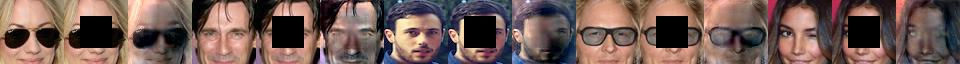
\includegraphics[width=\textwidth]{fig/inpaintings.jpg}
\caption{CelebA: Image in-paintings with STANLey}
\label{fig:anilaceleb}
\end{figure}

The improved STANLey paper will thus be improved in terms of baselines (3 additional ones presented in the rebuttal for CIFAR-10) and in terms of tasks: a) GMM toy example, 2) image generation on Flowers and CIFAR and 3) Image in-paintings.


\section{Quantized and Compressed sEM for Federated Learning}

The final method I am considering for solving federated optimization using the EM is the following:

\begin{algorithm}
\caption{Quantized and Compressed FL-SAEM with Periodic Statistics Averaging} \label{alg:flsaem2}
\begin{algorithmic}[1]
\State \textbf{Input}: Compression operator $\mathcal C(\cdot)$, number of rounds $R$, initial parameter $\theta_{0}$.
	\ForEach{$r=1$ to $R$}%
		\For{parallel for device $i \in D^{r}$}
		\State Set $\hat{\theta}^{(0,r)}_i = \hat{\theta}^{(r)}$. \algorithmiccomment{\textcolor{blue}{Initialize each worker with current global model}}
		\State Draw M samples $z_{i,m}^{(r)}$ under model $\hat{\theta}^{(r)}_i$ via Quantized LD: \algorithmiccomment{\textcolor{blue}{Local MCMC step}}
			\For{$k=1$ to $K$}
			\State Compute the quantized gradient of $\nabla \log p(z_i| y_i; \hat{\theta}^{(k)}_i)$: 
			$$g_i{(k,m)} = \mathsf{C}_{j}^{(\ell)}\left(\nabla_j f_{\theta_t}(z_i^{(k-1,m)}), \xi^{(k)}_{j}\right) \quad \textrm{where} \quad \xi^{(k)}_{j} \sim \mathcal{U}_{[a,b]} $$
			\State Sample the latent data using the following chain:
			\begin{equation}\notag
			z_i^{(k,m)} = z_i^{(k-1,m)} + \frac{\gamma_k}{2}  g_i{(k,m)} + \sqrt{\gamma_k}  \mathsf{B}_k ,
			\end{equation}
			\qquad\qquad\quad  where $\mathsf{B}_t$ denotes the Brownian motion and $m \in [M]$ denotes the MC sample.
			\EndFor
		\State Assign $\{ z_{i}^{(r,m} \}_{m=1}^M \leftarrow \{ z_i^{(K,m)} \}_{m=1}^M$.
		\State Compute $\tilde{S}_{i}^{(r+1)}$ and its \textbf{Top-$k$} variant $\ddot{S}_{i}^{(k+1)} = \mathcal C \left( \tilde{S}_{i}^{(k+1)}\right)$. \label{line:compute} \algorithmiccomment{\textcolor{blue}{Compressed Local Statistics}}
		\State Workers send local statistics $\tilde{S}_{i}^{(k+1)}$ to server. \algorithmiccomment{\textcolor{blue}{Single round of communication}}
          \EndFor
          \State Server computes \textbf{global model}: \algorithmiccomment{\textcolor{blue}{(Global) M-Step using Complete Statistics}}
$$
\hat{\theta}^{(r+1)} = \overline{\theta}( \ddot{S}^{(r+1)}) 
$$
\qquad where $\ddot{S}^{(r+1)} = (\ddot{S}_i^{(r+1)}, i \in D_r)$  and send global model back to the devices. 

    \EndForEach
  \end{algorithmic}
\end{algorithm}





\bibliographystyle{plain}
\bibliography{ref}


\end{document} 